\documentclass[12pt]{article}

%%%%%%%%%%%%%%%%%%%%%%%%%%%%%%%%%%%%%%%%%%%%%%%%%%%%%%%%%%%%%%%%%%%%%%%%%%%%%%%%
%                           Package preset for homework
%%%%%%%%%%%%%%%%%%%%%%%%%%%%%%%%%%%%%%%%%%%%%%%%%%%%%%%%%%%%%%%%%%%%%%%%%%%%%%%%
% Miscellaneous
\usepackage[margin=1in]{geometry}
\usepackage[utf8]{inputenc}
\usepackage{indentfirst}
\usepackage{blindtext}
\usepackage{graphicx}
\usepackage{xr-hyper}
\usepackage{hyperref}
\usepackage{enumitem}
\usepackage{color}
\usepackage{float}
% Math
\usepackage{latexsym}
\usepackage{amsfonts}
\usepackage{amssymb}
\usepackage{amsmath}
\usepackage{commath}
\usepackage{amsthm}
\usepackage{bbold}
\usepackage{bm}
% Physics
\usepackage{physics}
\usepackage{siunitx}
% Code typesetting
\usepackage{listings}
% Citation
\usepackage[authoryear]{natbib}
\usepackage{appendix}
\usepackage[capitalize]{cleveref}
% Title & name
\title{Homework}
\author{Tien Vo}
\date{\today}


%%%%%%%%%%%%%%%%%%%%%%%%%%%%%%%%%%%%%%%%%%%%%%%%%%%%%%%%%%%%%%%%%%%%%%%%%%%%%%%%
%                   User-defined commands and environments
%%%%%%%%%%%%%%%%%%%%%%%%%%%%%%%%%%%%%%%%%%%%%%%%%%%%%%%%%%%%%%%%%%%%%%%%%%%%%%%%
%%% Misc
\sisetup{load-configurations=abbreviations}
\newcommand{\due}[1]{\date{Due: #1}}
\newcommand{\hint}{\textit{Hint}}
\let\oldt\t
\renewcommand{\t}[1]{\text{#1}}

%%% Bold sets & abbrv
\newcommand{\N}{\mathbb{N}}
\newcommand{\Z}{\mathbb{Z}}
\newcommand{\R}{\mathbb{R}}
\newcommand{\Q}{\mathbb{Q}}
\let\oldP\P
\renewcommand{\P}{\mathbb{P}}
\newcommand{\LL}{\mathcal{L}}
\newcommand{\FF}{\mathcal{F}}
\newcommand{\HH}{\mathcal{H}}
\newcommand{\NN}{\mathcal{N}}
\newcommand{\ZZ}{\mathcal{Z}}
\newcommand{\RN}[1]{\textup{\uppercase\expandafter{\romannumeral#1}}}
\newcommand{\ua}{\uparrow}
\newcommand{\da}{\downarrow}

%%% Unit vectors
\newcommand{\xhat}{\vb{\hat{x}}}
\newcommand{\yhat}{\vb{\hat{y}}}
\newcommand{\zhat}{\vb{\hat{z}}}
\newcommand{\nhat}{\vb{\hat{n}}}
\newcommand{\rhat}{\vb{\hat{r}}}
\newcommand{\phihat}{\bm{\hat{\phi}}}
\newcommand{\thetahat}{\bm{\hat{\theta}}}

%%% Other math stuff
\providecommand{\units}[1]{\,\ensuremath{\mathrm{#1}}\xspace}
% Set new style for problem
\newtheoremstyle{problemstyle}  % <name>
        {10pt}                   % <space above>
        {10pt}                   % <space below>
        {\normalfont}           % <body font>
        {}                      % <indent amount}
        {\bfseries\itshape}     % <theorem head font>
        {\normalfont\bfseries:} % <punctuation after theorem head>
        {.5em}                  % <space after theorem head>
        {}                      % <theorem head spec (can be left empty, 
                                % meaning `normal')>

% Set problem environment
\theoremstyle{problemstyle}
\newtheorem{problemenv}{Problem}[section]
\newenvironment{problem}[1]{%
  \renewcommand\theproblemenv{#1}%
  \problemenv
}{\endproblemenv}
% Set lemma environment
\newenvironment{lemma}[2][Lemma]{\begin{trivlist}
\item[\hskip \labelsep {\bfseries #1}\hskip \labelsep {\bfseries #2.}]}{\end{trivlist}}
% Set solution environment
\newenvironment{solution}{
    \begin{proof}[Solution]$ $\par\nobreak\ignorespaces
}{\end{proof}}
\numberwithin{equation}{problemenv}

%%% Page format
\setlength{\parindent}{0.5cm}
\setlength{\oddsidemargin}{0in}
\setlength{\textwidth}{6.5in}
\setlength{\textheight}{8.8in}
\setlength{\topmargin}{0in}
\setlength{\headheight}{18pt}

%%% Code environments
\definecolor{dkgreen}{rgb}{0,0.6,0}
\definecolor{gray}{rgb}{0.5,0.5,0.5}
\definecolor{mauve}{rgb}{0.58,0,0.82}
\lstset{frame=tb,
  language=Python,
  aboveskip=3mm,
  belowskip=3mm,
  showstringspaces=false,
  columns=flexible,
  basicstyle={\small\ttfamily},
  numbers=none,
  numberstyle=\tiny\color{gray},
  keywordstyle=\color{blue},
  commentstyle=\color{dkgreen},
  stringstyle=\color{mauve},
  breaklines=true,
  breakatwhitespace=true,
  tabsize=4
}
\lstset{
  language=Mathematica,
  numbers=left,
  numberstyle=\tiny\color{gray},
  numbersep=5pt,
  breaklines=true,
  captionpos={t},
  frame={lines},
  rulecolor=\color{black},
  framerule=0.5pt,
  columns=flexible,
  tabsize=2
}


\title{Homework 3: Phys 7310 (Fall 2021)}

\begin{document}

\maketitle

%%%%%%%%%%%%%%%%%%%%%%%%%%%%%%%%%%%%%%%%%%%%%%%%%%%%%%%%%%%%%%%%%%%%%%%%%%%%%%%%
\begin{problem}{3.1}[A plate with a half-sphere]~\\
    \begin{figure}[h]
        \centering
        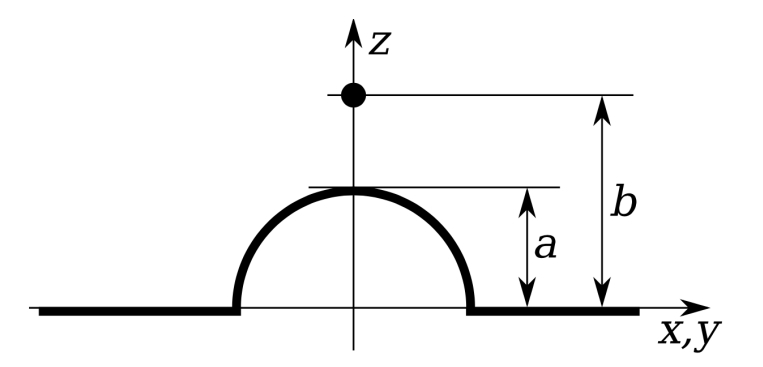
\includegraphics[width=0.5\textwidth]{hw3_p1.jpg}
    \end{figure}
An infinite grounded conducting plate has a bulge in form of a haf-sphere with
radius $a$. A point charge $q$ is put on the symmetry axis of the system at a
distance $b>a$ from the center of the half-sphere (see figure). Using the method
of image, calculate the potential $\Phi$ above the plate, the force on the point
charge $q$, and the total charge induced on the half-sphere.
\end{problem}
%%%%%%%%%%%%%%%%%%%%%%%%%%%%%%%%%%%%%%%%%%%%%%%%%%%%%%%%%%%%%%%%%%%%%%%%%%%%%%%%
\begin{problem}{3.2}[A line charge]
In this problem, we consider an infinite line with a constant linear charge
density $\lambda$ (charge per unit length). Let the line charge sit at the
origin $(x,y)=(0,0)$ in the $xy$-plane, and stretch infinitely in both
directions along the $z$-axis.

Draw an appropriate Gaussian surface and find the electric field a distance $r$
away from the line charge. Show that a potential for this electric field takes
the form
\begin{equation}
    \Phi(\vb{x})=\alpha\ln\frac{r}{R} 
\end{equation}
where $\alpha$ is a constant you should determine in terms of $\lambda$ and
other things, and $R$ is a \textit{totally arbitrary} constant with units of
length that we include to make the units in the log dimensionless; explain why
$R$ drops out of physically measurable quantities. Finally, if there is another
line charge with linear charge density $\lambda'$ a distance $r$ away from the
first charge, find the force per unit length experienced by this second line
charge.
\end{problem}
%%%%%%%%%%%%%%%%%%%%%%%%%%%%%%%%%%%%%%%%%%%%%%%%%%%%%%%%%%%%%%%%%%%%%%%%%%%%%%%%
\begin{problem}{3.3}[Line charges and images]
A straight line charge with constant linear charge density $\lambda$ is located
perpendicular to the $xy$-plane in the first quadrant at $(x_0,y_0)$. The
intersecting planes $x=0$, $y\geq0$, and $y=0,x\geq0$ are conducting boundary
surfaces held at zero potential. Consider the potential, fields, and surface
charges in the first quadrant.

(a) The well-known potential for an isolated line charge at $(x_0,y_0)$ is
$\Phi(x,y)=(\lambda/4\pi\epsilon_0)\ln(R^2/r^2)$ where $r^2=(x-x_0)^2+(y-y_0)^2$
and $R$ is a constant. Determine the expression for the potential of the line
charge in the presence of the intersecting planes. Verify explicitly that the
potential and the tangential eectric field vanish on the boundary surfaces.

(b) Determine the surface charge density $\sigma$ on the plane $y=0,x\geq0$.
Plot $\sigma/\lambda$ versus $x$ for
$(x_0=2,y_0=1),(x_0=1,y_0=1),(x_0=1,y_0=2)$.

(c) Show that the total charge (per unit length in $z$) on the plane $y=0,x\geq
0$ is
\begin{equation}
    Q_x=-\frac2\pi\lambda\tan^{-1}\qty(\frac{x_0}{y_0}) 
\end{equation}
What is the total charge on the plane $x=0$?

(d) Show that far from the origin [$\rho\gg\rho_0$, where $\rho=\sqrt{x^2+y^2}$
and $\rho_0=\sqrt{x_0^2+y_0^2}$] the leading term in the potential is
\begin{equation}
    \Phi\to\Phi_{\text{asym}}=\frac{4\lambda}{\pi\epsilon_0}\frac{(x_0y_0)(xy)}{\rho^4} 
\end{equation}
Interpret.
\end{problem}
%%%%%%%%%%%%%%%%%%%%%%%%%%%%%%%%%%%%%%%%%%%%%%%%%%%%%%%%%%%%%%%%%%%%%%%%%%%%%%%%
\begin{problem}{3.4}[Green's function in Cartesian coordinates]
(a) Show that the Green function $G(x,y;x',y')$ appropriate for Dirichlet
boundary conditions for a square two-dimensional region, $0\leq x\leq1,0\leq
y\leq1$, has an expansion
\begin{equation}
    G(x,y;x',y')=2\sum_{n=1}^\infty g_n(y,y')\sin(n\pi x)\sin(n\pi x') 
\end{equation}
where $g_n(y,y')$ satisfies
\begin{equation}
    \qty(\frac{\partial^2}{\partial y'^2}-n^2\pi^2)g_n(y,y')
    =-4\pi\delta(y'-y)
    \qquad\text{and}\qquad
    g_n(y,0)=g_n(y,1)=0
\end{equation}

(b) Taking for $g_n(y,y')$ appropriate linear combinations of $\sinh\qty(n\pi
y')$ and $\cosh(n\pi y')$ in the two regions, $y'<y$ and $y'>y$, in accord with
the boundary conditions and the discontinuity in slope required by the source
delta function, show that the explicit form of $G$ is
\begin{equation}
    G(x,y;x',y')=8\sum_{n=1}^\infty
        \frac{1}{n\sinh(n\pi)}\sin(n\pi x)\sin(n\pi x')\sinh(n\pi
        y_<)\sinh\qty[n\pi\qty(1-y_>)]
\end{equation}
where $y_<(y_>)$ is the smaller (larger) of $y$ and $y'$.
\end{problem}
%%%%%%%%%%%%%%%%%%%%%%%%%%%%%%%%%%%%%%%%%%%%%%%%%%%%%%%%%%%%%%%%%%%%%%%%%%%%%%%%

\end{document}
